\documentclass{article}

\usepackage[letterpaper, portrait, margin=1.5in]{geometry}

\usepackage{fancyhdr}
\usepackage{ragged2e}
\usepackage{graphicx}
\usepackage{caption}
\usepackage{amsmath}
\usepackage{rotating}

\usepackage{listings}
\usepackage{color}

\definecolor{dkgreen}{rgb}{0,0.6,0}
\definecolor{gray}{rgb}{0.5,0.5,0.5}
\definecolor{mauve}{rgb}{0.58,0,0.82}

\lstset{frame=tb,
  language=Java,
  aboveskip=3mm,
  belowskip=3mm,
  showstringspaces=false,
  columns=flexible,
  basicstyle={\small\ttfamily},
  numbers=none,
  numberstyle=\tiny\color{gray},
  keywordstyle=\color{blue},
  commentstyle=\color{dkgreen},
  stringstyle=\color{mauve},
  breaklines=true,
  breakatwhitespace=true,
  tabsize=4
}

\setcounter{secnumdepth}{1}

\usepackage{chngcntr}
\counterwithin{figure}{section}

\renewcommand*{\thepage}{C\arabic{page}}

\pagestyle{fancy}
\lhead{ACME Robotics}
\chead{\#8367}
\rhead{\ifcontents Contents \else Week \thesection \fi}

\newif\ifcontents
\contentstrue

\makeatletter
\renewcommand{\@seccntformat}[1]{}
\makeatother
\begin{document}

\subsection{Lift Cross brace and LED side plates}
%! Discussing an alternative cross brace and decorative side plates.
Most of the lift had been completed and one of the only things left was to create the cross brace at the top of the lift. The cross brace was necessary because without it the entire lift would wobble five to ten degrees when at max height. While Aidan created the brackets on the side of the lift to hold the cross brace, Aidan, Kelly and Oren discussed what they wanted to make the cross brace to be made out of. They decided that instead of just the metal plate running across they wanted to make the cross brace out of cast acrylic so that they could engrave patterns into the acrylic and light it up with LED's.They decided to do this with the acrylic instead of poly-carbonate because the poly-carbonate would melt a little when engraved. They then realized that they could also create similar illuminated plates on the side of the robot. However before these plates could be cut the designs needed to be created. Since this might take a few days, Aidan created a temporary cross brace that would serve until then.

\subsection{Adjusting the angle of the diverter cartridge}
%! The diverter cartridge angle needs to be changed to allow for cubes to fall out.
When most of the intake had been completed, Kelly, Aidan and Oren decided to fully test the diverter and lift. One thing they realized is that if there was a cube in the back of the diverter, the cube would not gain enough speed to roll out. They decided that the angle of the diverter needed to be increased to allow for this. Aidan fixed this problem by slightly cutting into the arm from the diverter to the servo which allowed the diverter to tilt farther as shown in figure \ref{fig:Cutout}. Aidan tested this and the cube gained sufficient speed with the new angle.

\begin{figure}
    \centering
    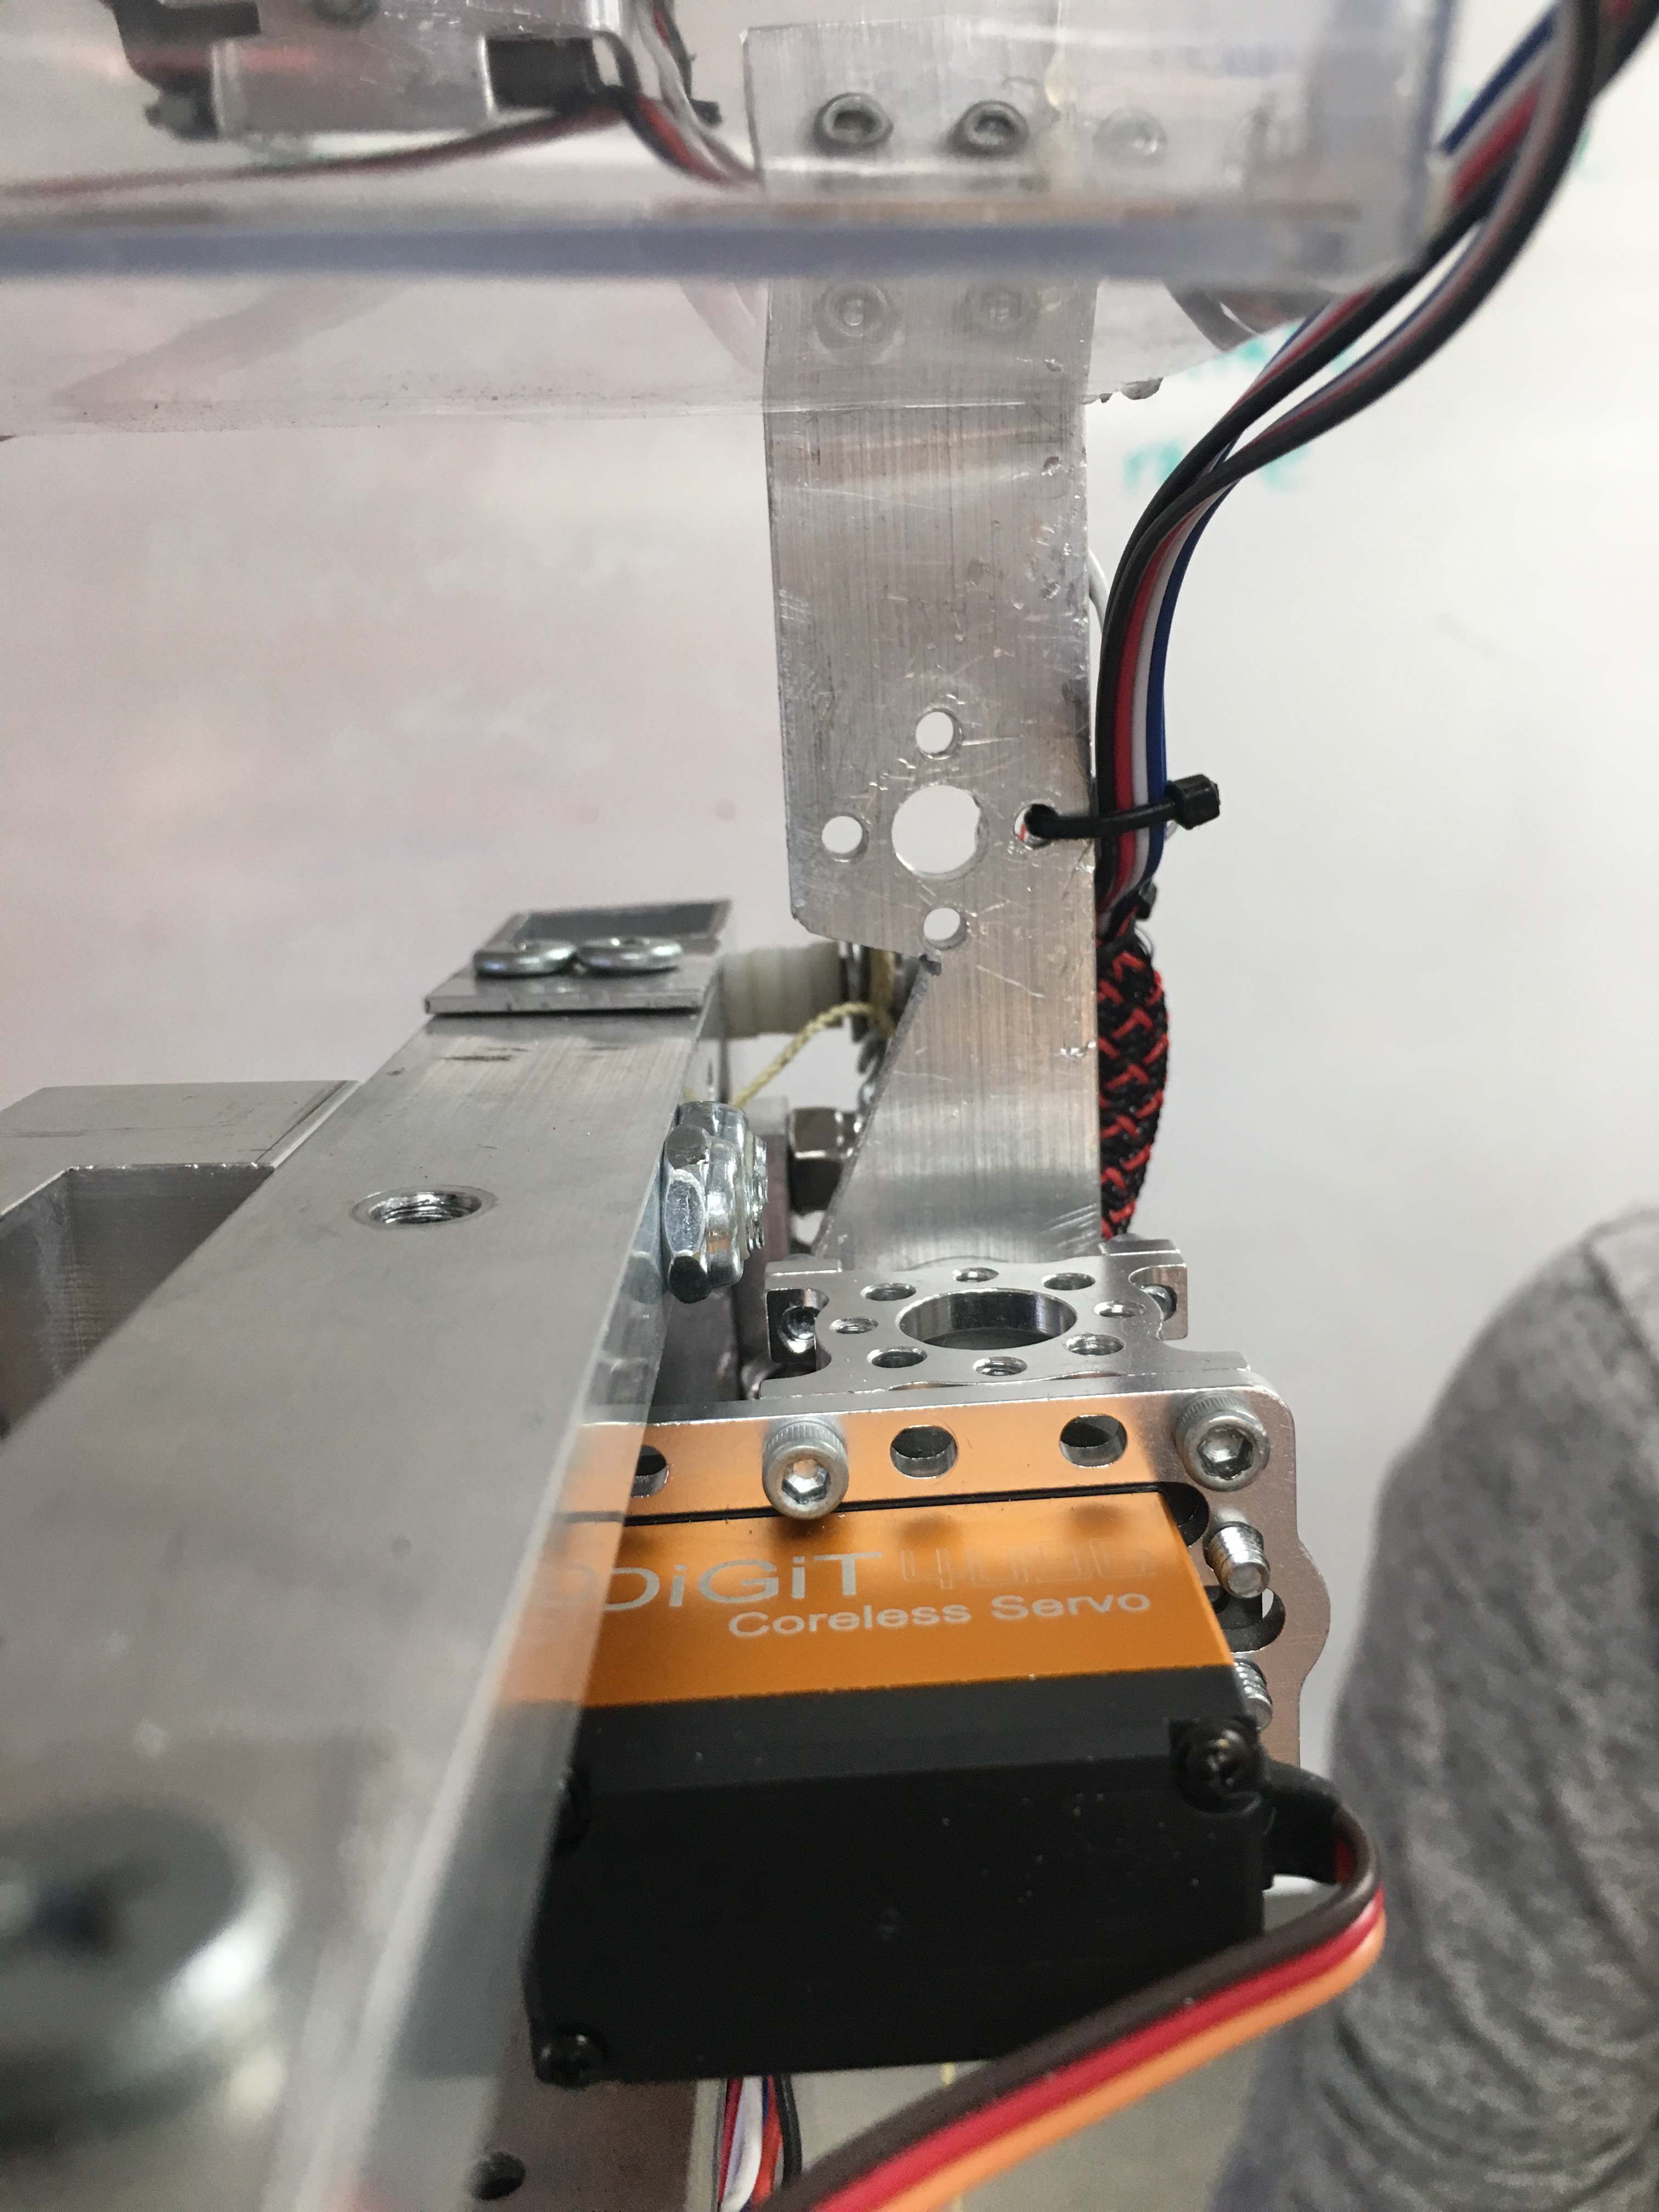
\includegraphics[height=6cm]{19_01-07/images/DiverterAngleCut.jpg}
    \caption{The cut to increase diverter angle}
    \label{fig:Cutout}
\end{figure}

\end{document}